\documentclass[10pt, a4paper]{report}

\usepackage{tocloft} % para cambiar formato de \tableofcontents
\usepackage{titlesec} % para cambiar formato de los titulos
\usepackage{amsmath, amssymb, amsthm, mathtools, esint} % Paquetes de simbolos matematicos
\usepackage{xcolor}
\usepackage[skip=20pt, indent=0pt]{parskip} 
\usepackage[margin=3cm]{geometry}
\usepackage[spanish, shorthands=off]{babel} % Disable shorthands to prevent conflicts
\usepackage{chngcntr} % para cambiar los contadores
\usepackage{hyperref} % para hyperlinks asociados al documento
\usepackage{pgfplots} % para graficos 
\pgfplotsset{compat=1.18}
\usepackage{tikz}
\usepgfplotslibrary{fillbetween}
\usetikzlibrary{patterns, shapes}
\usetikzlibrary{arrows.meta, decorations.pathmorphing, positioning}

% para graficar flechas en curvas cerradas
\xdef\Rad{2}
\newcommand{\ARW}[2][]{%
    \foreach \ang in {#2}{%
        \draw[#1] (\ang:\Rad)--(\ang+1:\Rad) ;
    }
}
% simbolo final de teorema, definicion, corolario, etc.
\newcommand{\final}{\hfill$\diamond$}
\newcommand{\finalmath}{\tag*{$\diamond$}}
% numeros reales
\renewcommand{\Re}{\mathbb {R}}
% derivadas parciales
\newcommand{\partialx}{\frac{\partial}{\partial x}}
\newcommand{\partialy}{\frac{\partial}{\partial y}}
\newcommand{\partialz}{\frac{\partial}{\partial z}}
% numeros romanos
\newcommand*{\rom}[1]{\expandafter\@slowromancap\romannumeral #1@}

%%%%%%%%%%%%%%%%%%%%%%%%%%%%
\renewcommand{\contentsname}{Indice}
\renewcommand{\listfigurename}{Lista de Figuras}
\renewcommand{\listtablename}{Lista de Tablas}
\renewcommand{\bibname}{Bibliograf\'{\i}a}
\renewcommand{\indexname}{Indice}
\renewcommand{\figurename}{Figura}
\renewcommand{\tablename}{Tabla}
\renewcommand{\partname}{Parte}
\renewcommand{\chaptername}{Cap\'{\i}tulo}
\renewcommand{\appendixname}{Ap\'endice}
\renewcommand{\abstractname}{Resumen}
%%%%%%%%%%%%%%%%%%%%%%%%%%%%

%%%%%%%%%%%%%%%%%%%%%%%%%%%%%%%%
%  Teoremas y proposiciones
%%%%%%%%%%%%%%%%%%%%%%%%%%%%%%%%%
\theoremstyle{definition} % Para que el texto no aparezca en italicas
\newtheorem{question}{Ejercicio}
\newtheorem{solution}{Solución}
\newtheorem{theorem}{Teorema}[section]
\newtheorem{corollary}{Corolario}[section]
\newtheorem{definition}{Definic\'on}[section]
\newtheorem{propertie}{Propiedad}[section]
\newtheorem{example}{Ejemplo}[section]

% Provide commands for \autoref
\providecommand*{\questionautorefname}{Ejercicio}
\providecommand*{\solutionautorefname}{Solución}
\providecommand*{\theoremautorefname}{Teorema}
\providecommand*{\corollaryautorefname}{Corolario}
\providecommand*{\definitionautorefname}{Definición}
\providecommand*{\propertieautorefname}{Propiedad}
\providecommand*{\exampleautorefname}{Ejemplo}

% Para que se resetee el contador en cada seccion
\counterwithin*{solution}{subsubsection}
\counterwithin*{question}{subsubsection}

% \newtheorem{teo}{Teorema}[section]
% \newtheorem{prop}[teo]{Proposici\'on}
% \newtheorem{lema}[teo]{Lema}
% \newtheorem{obs}[teo]{Observaci\'on}
% \newtheorem{exmpl}[teo]{Ejemplo}
% \newtheorem{coro}[teo]{Corolario}
% \newtheorem{comen}[teo]{Comentario}
% \newtheorem{conje}[teo]{Conjetura}
% \theoremstyle{definition}
% \newtheorem{definition}[teo]{Definici\'on}
% \newtheorem{propertie}[teo]{Propiedad}

\spanishdecimal{.}

% ajuste formato capitulos
\titleformat{\chapter}[display]
  {\normalfont\fontsize{14}{16}\selectfont\bfseries}{\vspace{-4cm}}{0pt}{}[\vspace{-1cm}]

% ajuste formato secciones
\titleformat{\section}
  {\normalfont\fontsize{12}{14}\selectfont\bfseries}{\thesection}{1em}{}

% ajuste formato indice
\renewcommand{\cfttoctitlefont}{\normalfont\Large\bfseries}
\renewcommand{\cftbeforetoctitleskip}{-.5cm}


%----------------------------------------------------------------
%----------------------------------------------------------------
\begin{document}


\begin{definition} [Grafica de $f$] 
\label{def:grafica}
 \mbox{}
 
Sea $f: A\subseteq\Re^n\rightarrow\Re$; se define la gráfica de $f$; y se nota $graf(f)$; a
 \[
graf(f)=\{(x_1,x_2,...,x_n,x_{n+1})\in\Re^{n+1} \backslash (x_1,x_2,...,x_n)=A \land f(x_1,x_2,...,x_n)=x_{n+1} \}
 \]

Para interpretar esta definición, podemos realizar un recuerdo a Análisis matemático 1, donde la $graf (f)$ de una funcion $f: A\subseteq\Re\rightarrow\Re$ se define como
 \[
graf(f)=\{(x,y)\in\Re^2 \backslash x\subseteq A=Dom(f) \land y=f(x) \}
 \]
Planteamos de ejemplo: $f=x^2-1$ donde podemos ver que para cada valor de $x$, existe un único valor de y. Para encontrar la gráfica de la funcion, nos fijamos utilizando la siguiente tabla
\begin{table}[h!]
\centering
\begin{tabular}{|c|c|}
\hline
\textbf{$x$} & \textbf{$f(x)$}  \\ \hline
0             & -1                         \\ \hline
1             & 0                        \\ \hline
-1             & 0                          \\ \hline
2             & 3                          \\ \hline
-2             & 3                          \\ \hline
\end{tabular}
\caption{Valores de $f(x)$}
\label{tabla1}
\end{table}
\begin{figure}[h!] % El entorno figure te permite incluir imágenes
    \centering
    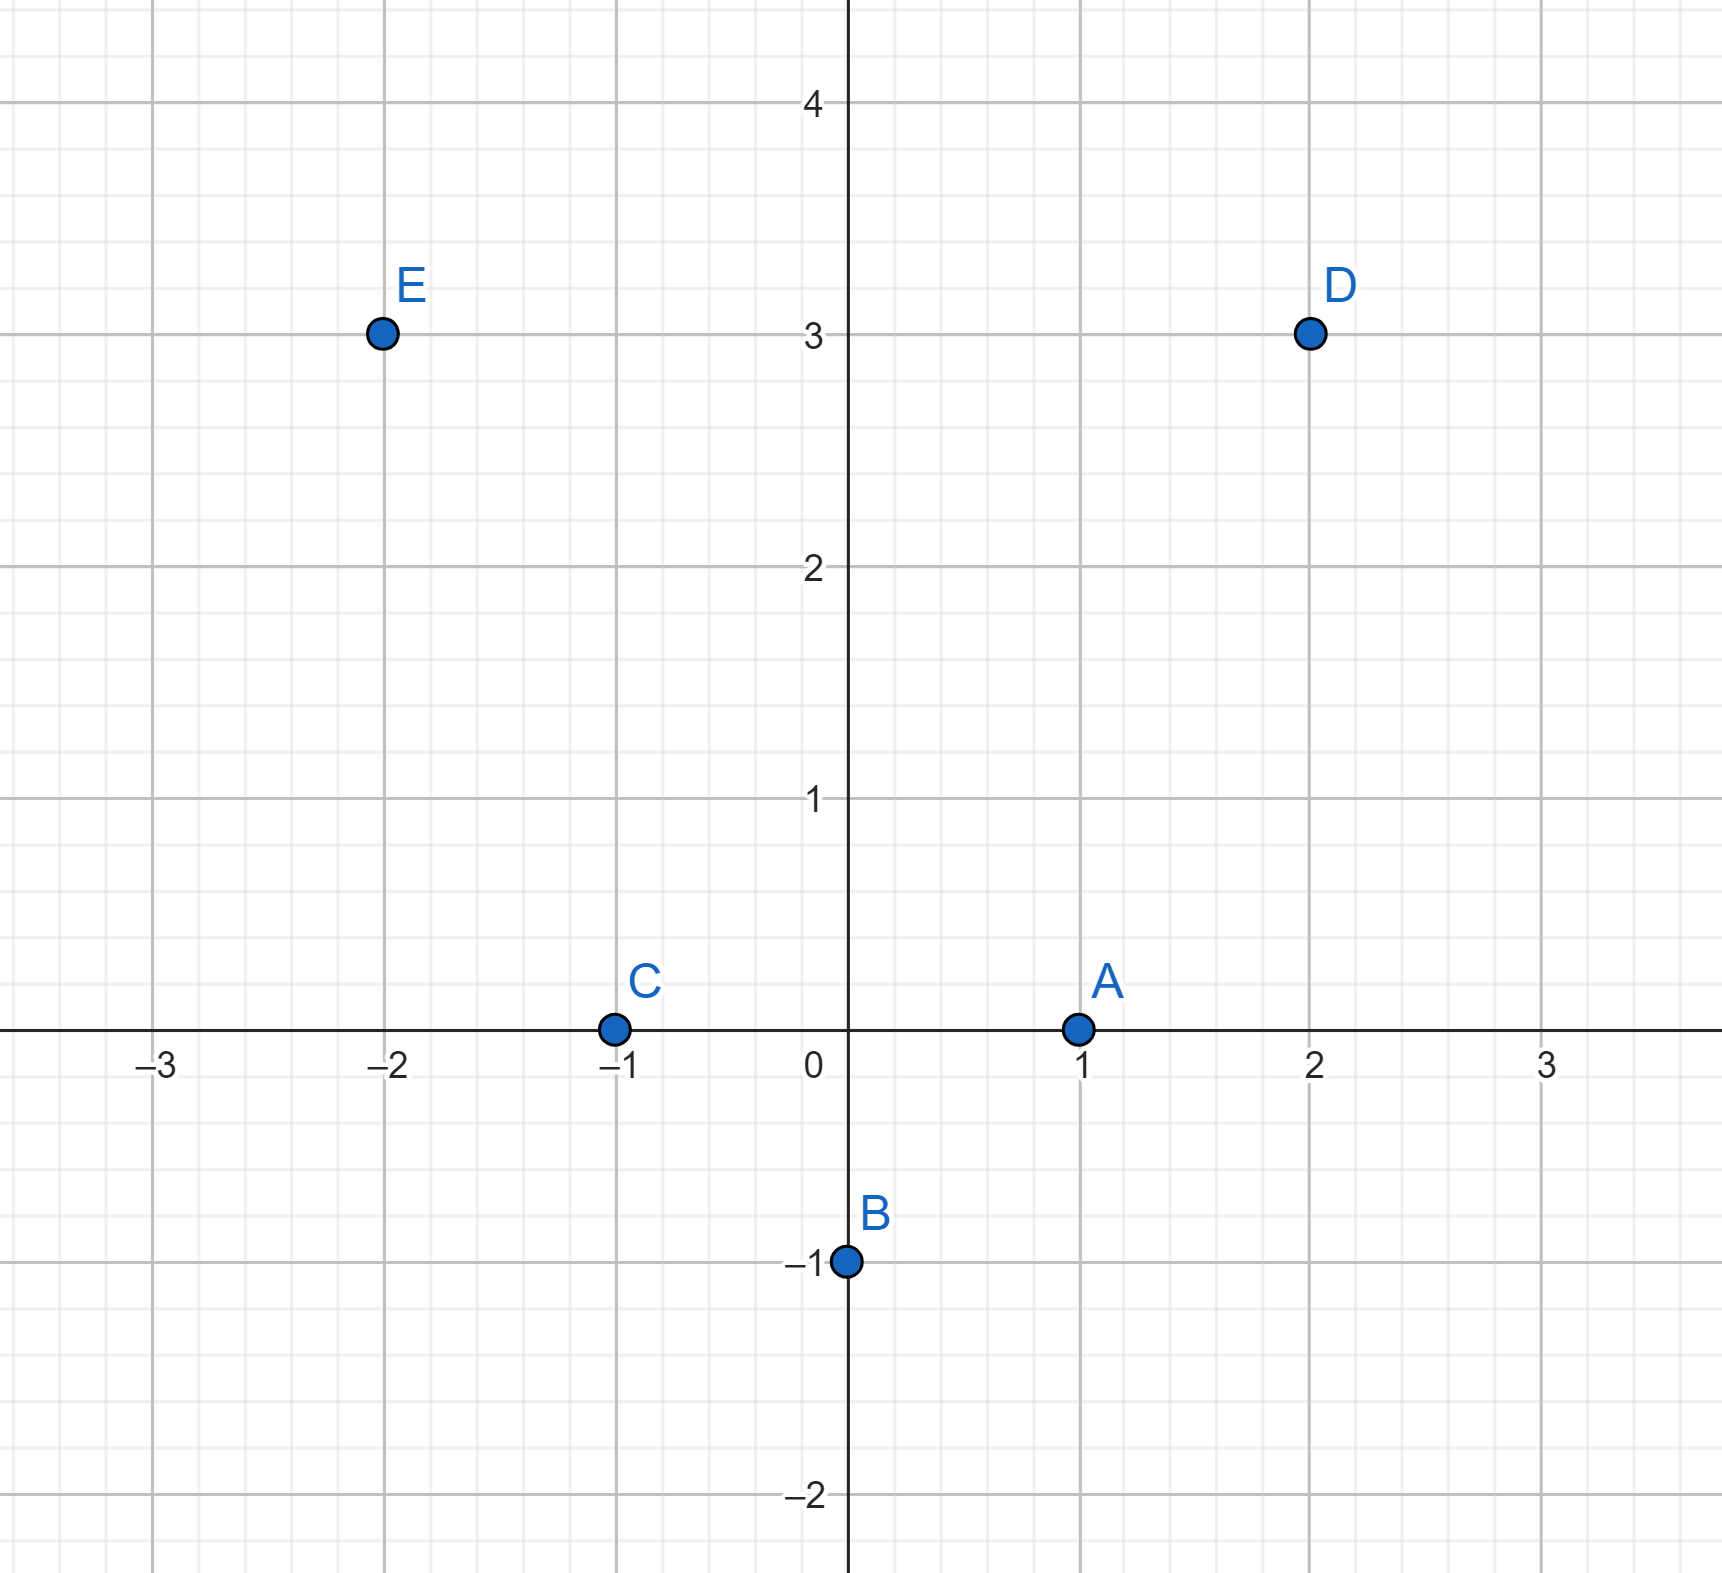
\includegraphics[width=0.34\textwidth]{Puntos_grafica.png} % Cambia esta ruta por la ubicación de tu imagen
    \caption{Puntos de tabla 1.}
    \label{fig:ejemplo} % Etiqueta para hacer referencia a la imagen
\end{figure}


De esta manera, se puede empezar a representar la grafica de $f$
\begin{figure}[h!] % El entorno figure te permite incluir imágenes
    \centering
    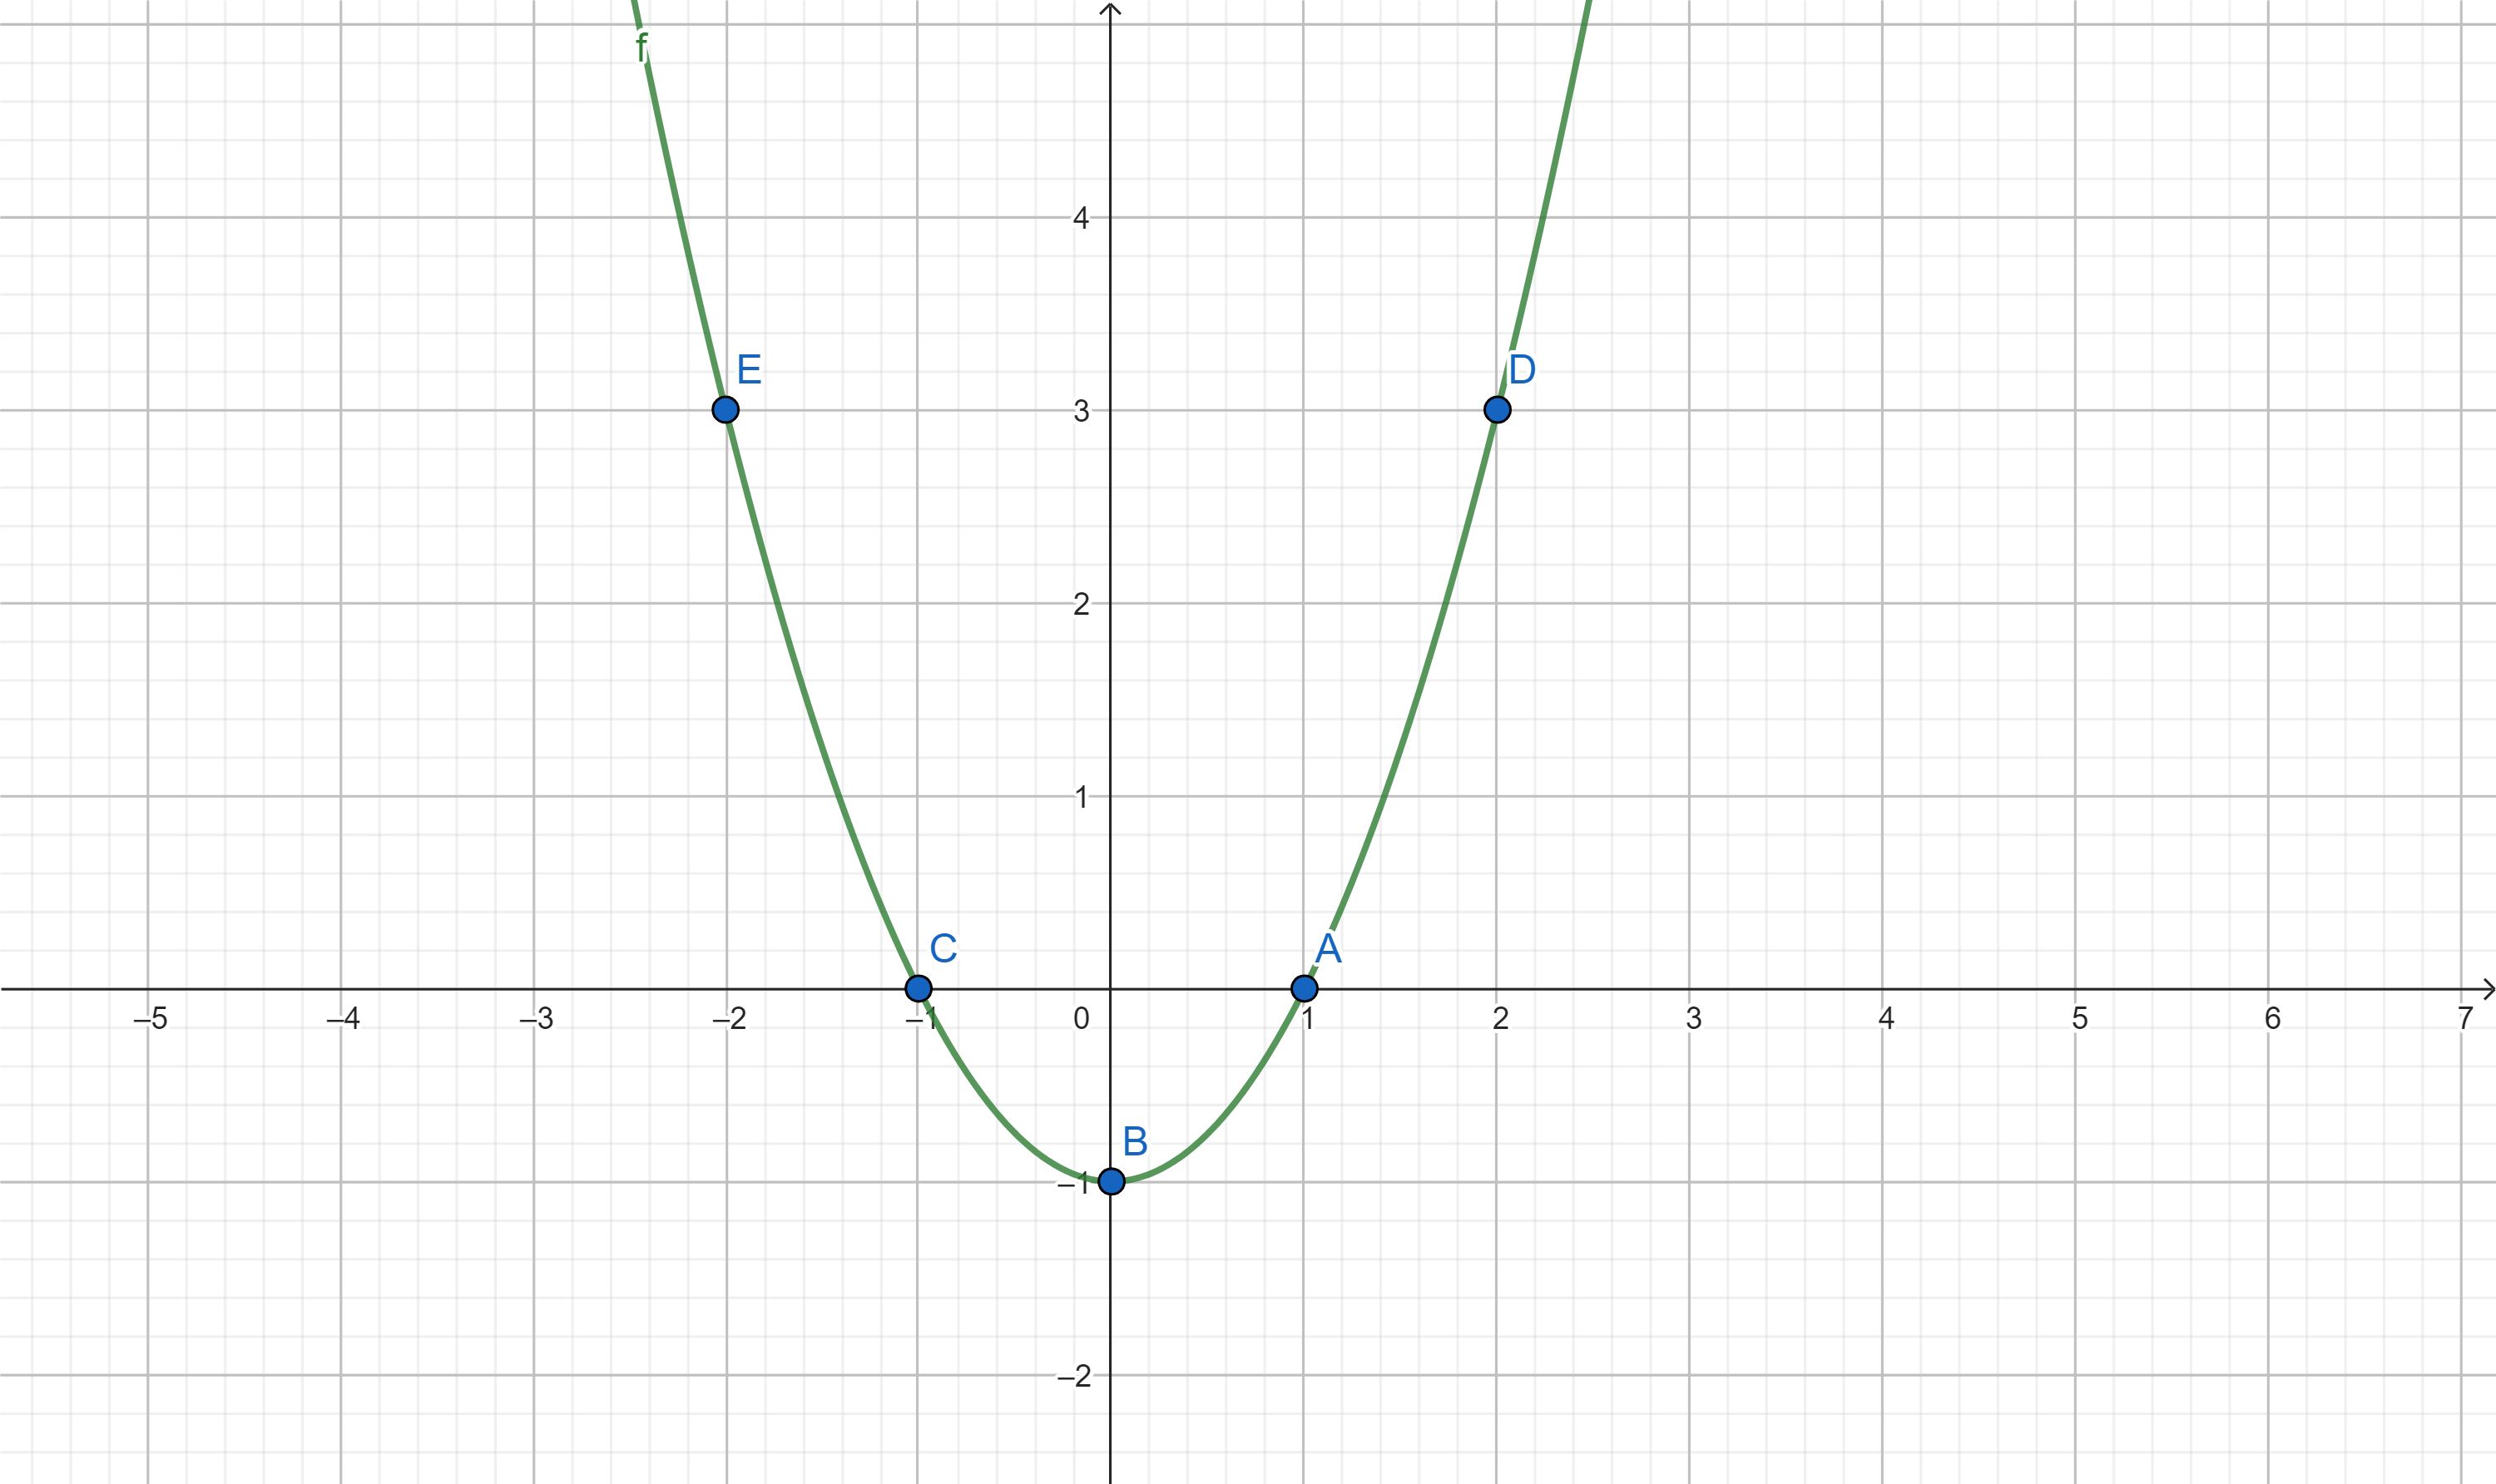
\includegraphics[width=0.5\textwidth]{r2_grafica.png} % Cambia esta ruta por la ubicación de tu imagen
    \caption{Grafica de $f(x)$.}
    \label{fig:ejemplo} % Etiqueta para hacer referencia a la imagen
\end{figure}
\end{definition}
Ahora, podemos pensar en las mismas definiciones pero analizandolas en $\Re^{3}$, donde la $graf (h)$ de una funcion $h: A\subseteq\Re^{2}\rightarrow\Re$ se define como
 \[
graf(h)=\{(x,y,z)\in\Re^2 \backslash (x,y)\subseteq A=Dom(h) \land z=h(x,y) \}
 \]
En este curso, se analizaran las graficas de funciones en  $\Re^{3}$. Analizamos un ejemplo, tomando $h(x,y)=x^2+y^2$.
Para la función , que representa un paraboloide, los conjuntos de nivel están dados por $h(x,y)=c$, que son círculos concéntricos en el plano xy. Graficando esta función en 3D, podemos ver una superficie parabólica, donde los conjuntos de nivel son las proyecciones de estas circunferencias a diferentes alturas en el eje z y con radio creciente.
\begin{figure}[h!] % El entorno figure te permite incluir imágenes
    \centering
    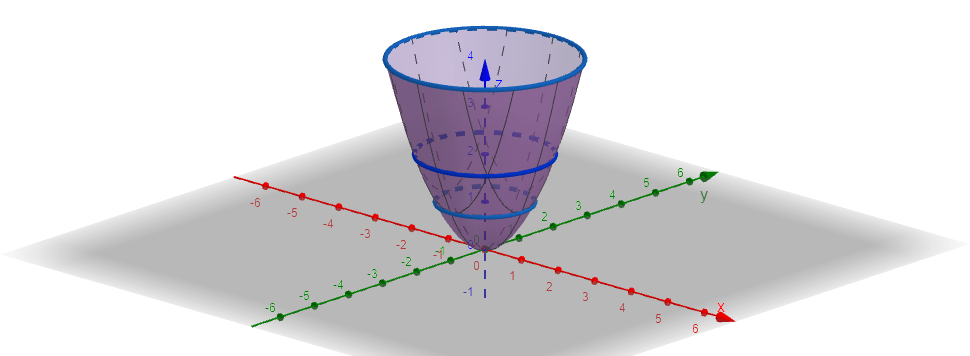
\includegraphics[width=1\textwidth]{r3_grafica.png} % Cambia esta ruta por la ubicación de tu imagen
    \caption{\small{ Gráfica de h y conjuntos de nivel tomando 
    c=\{1,2,4}\}}
    \label{fig:ejemplo} % Etiqueta para hacer referencia a la imagen
\end{figure}

\end{document}
